\documentclass{article}
\usepackage[margin=1in]{geometry}
\usepackage{graphicx}
\usepackage{multicol}

\title{Project 2\\Tulsa Weather Prediction using a Feed-Forward Neural Network with a Sigmoid Activation Function and Supervised Learning Techniques}

\author{Christian Mann, Steven Reed}

\begin{document}

\maketitle

\begin{multicols}{2}

\begin{abstract}
In this paper we develop our own Feed-Forward Neural Network based off of previous examples found in the book and on the Internet. The Neural Network features Backpropogation for supervised learning. We then use it to approximate various functions. First we approximate the simple XOR function, then we attempt to approximate the behavior of weather in Tulsa, OK.
\end{abstract}

\section{Introduction}

A Neural Network is an abstract concept derived from studies in neuroscience. The general concept behind the structure of a Neural Network is simple to understand, yet it proves to be an incredibly difficult challenge to create a network of use. The purpose of a Neural Network is, in short, to approximate a function. Sometimes this function is known explicitly, but is difficult or expensive to compute. Other times the function cannot be explicitly known, but we can gather empirical data relating to the function. With a Neural Network, the goal is to approximate these functions using what information we have available about them.

There are two main techniques in developing the structure of a Neural Network. One technique is called Supervised Learning, in which the Network is ``trained'' by means of giving it example inputs and outputs from the function we want it to approximate. After pouring over the examples over and over, the Network (hopefully) becomes well equipped at evaluating those inputs, as well as similar ones. It does this by making many small changes to the weights associated with the edges in the network using a method known as ``backpropogation''. The second popular method for constructing a Neural Network is known as Unsupervised Learning; we do not use any Unsupervised Learning techniques in this project.

We began by researching existing Neural Networks. There are many available, and all have a varying set of features and capabilities. Many implementations take advantage of your computer's GPU to parallelize the computations. The most simplistic example Network we could find, though, was a javascript implementation known as Brain.js. We used Brain.js as a guide for creating our own Neural Network in C++ with the hopes of performing faster at a lower level.


\section{Conclusion}

\end{multicols}

\begin{figure}[tb]
	\begin{center}
		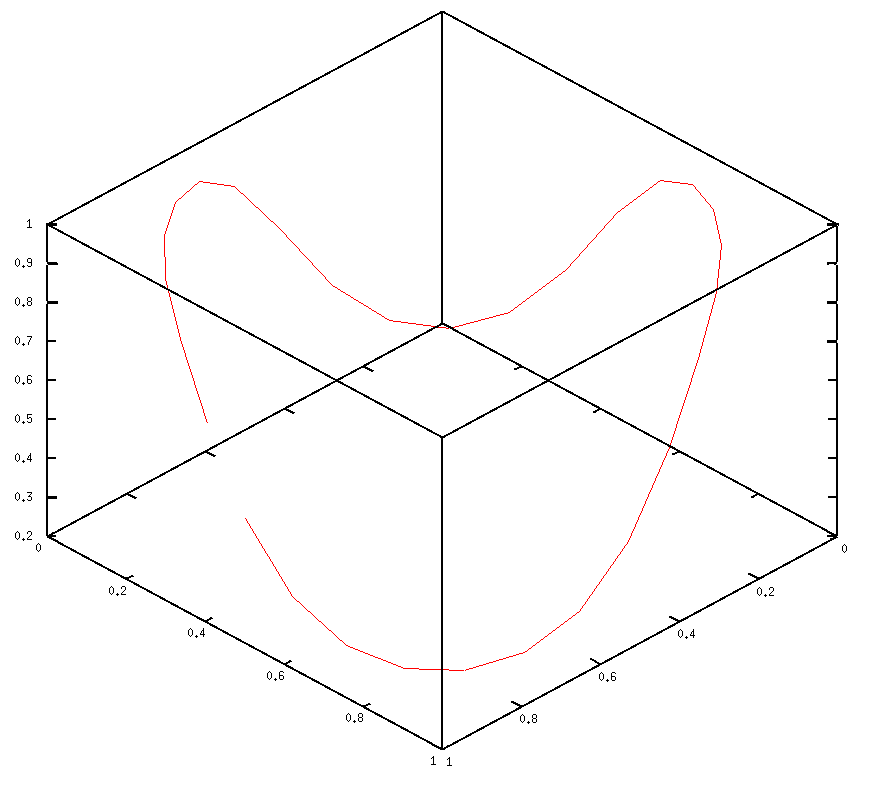
\includegraphics[scale=0.5]{img/xor1}
	\end{center}
	\caption{XOR function}
	\label{fig:xor1}
\end{figure}

\begin{figure}[tb]
	\begin{center}
		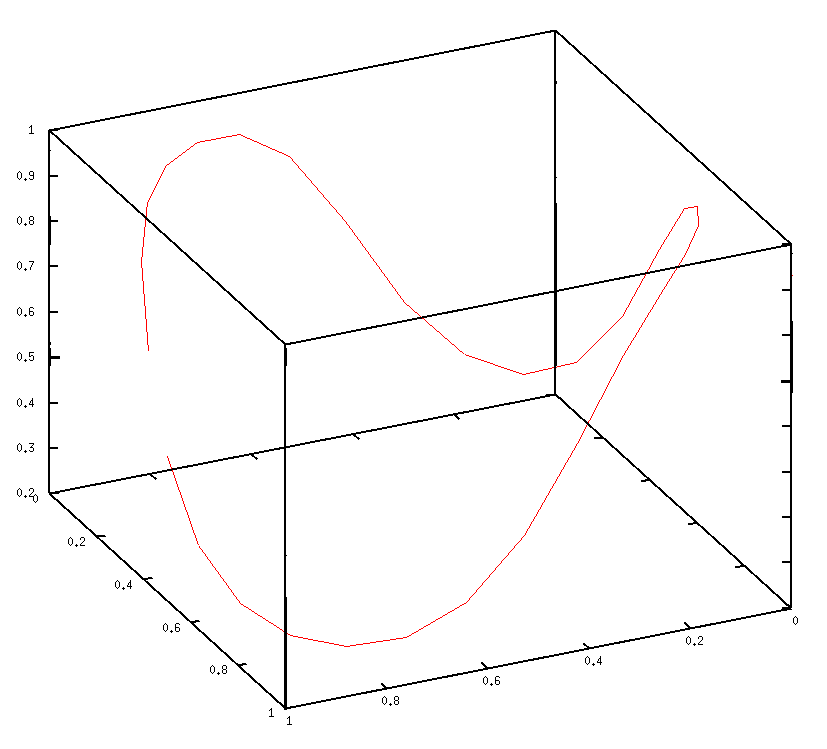
\includegraphics[scale=0.5]{img/xor2}
	\end{center}
	\caption{XOR Function}
	\label{fig:xor2}
\end{figure}


\end{document}

% citations:
% trappenberg
% brain.js
% weather data
% wolfram alpha/mathematica